% Preamble templated from Mihir-Divyansh/Course-Setup
%iffalse
\let\negmedspace\undefined
\let\negthickspace\undefined
\documentclass[journal,12pt,onecolumn]{IEEEtran}
\usepackage{cite}
\usepackage{amsmath,amssymb,amsfonts,amsthm}
\usepackage{algorithmic}
\usepackage{graphicx}
\usepackage{textcomp}
\usepackage{xcolor}
\usepackage{txfonts}
\usepackage{listings}
\usepackage{enumitem}
\usepackage{mathtools}
\usepackage{gensymb}
\usepackage{comment}
\usepackage[breaklinks=true]{hyperref}
\usepackage{tkz-euclide}
\usepackage{listings}
\usepackage{gvv}
%\def\inputGnumericTable{}
\usepackage[latin1]{inputenc}
\usepackage{color}
\usepackage{array}
\usepackage{longtable}
\usepackage{calc}
\usepackage{multirow}
\usepackage{hhline}
\usepackage{ifthen}
\usepackage{lscape}
\usepackage{tabularx}
\usepackage{array}
\usepackage{float}
\usepackage{caption}
\usepackage{multicol}

\newtheorem{theorem}{Theorem}[section]
\newtheorem{problem}{Problem}
\newtheorem{proposition}{Proposition}[section]
\newtheorem{lemma}{Lemma}[section]
\newtheorem{corollary}[theorem]{Corollary}
\newtheorem{example}{Example}[section]
\newtheorem{definition}[problem]{Definition}
\newcommand{\BEQA}{\begin{eqnarray}}
\newcommand{\EEQA}{\end{eqnarray}}
%\newcommand{\define}{\stackrel{\triangle}{=}}
\theoremstyle{remark}
%\newtheorem{rem}{Remark}

% Marks the beginning of the document
\begin{document}
\bibliographystyle{IEEEtran}
\vspace{3cm}

\title{Assignment 2: 1.10.18}
\author{EE25BTECH11055 - Subhodeep Chakraborty}
\maketitle
\hrulefill
\bigskip

\renewcommand{\thefigure}{\theenumi}
\renewcommand{\thetable}{\theenumi}

\textbf{Question:}\par
Write the direction ratios of the vector $\vec{a} = \hat{\imath} + \hat{\jmath} - \hat{k}$ and hence calculate its direction cosines. \par
\textbf{Solution:}\par

Given vector:
\begin{align}
 \vec{a} &= \myvec{1 \\ 1 \\ -1}
\end{align}
$\therefore$ The direction ratios are 1, 1 and -1. \\
Now,
\begin{align*}
\norm{\vec{a}} = \sqrt{3} \\
\implies \frac{\vec{a}}{\norm{\vec{a}}} = \myvec{\frac{1}{\sqrt{3}} \\ \frac{1}{\sqrt{3}} \\ \frac{-1}{\sqrt{3}}}
\end{align*}
Thus we see that the direction cosines are $1/\sqrt{3}$, $1/\sqrt{3}$ and $-1/\sqrt{3}$.
\begin{figure}[H]
    \centering
    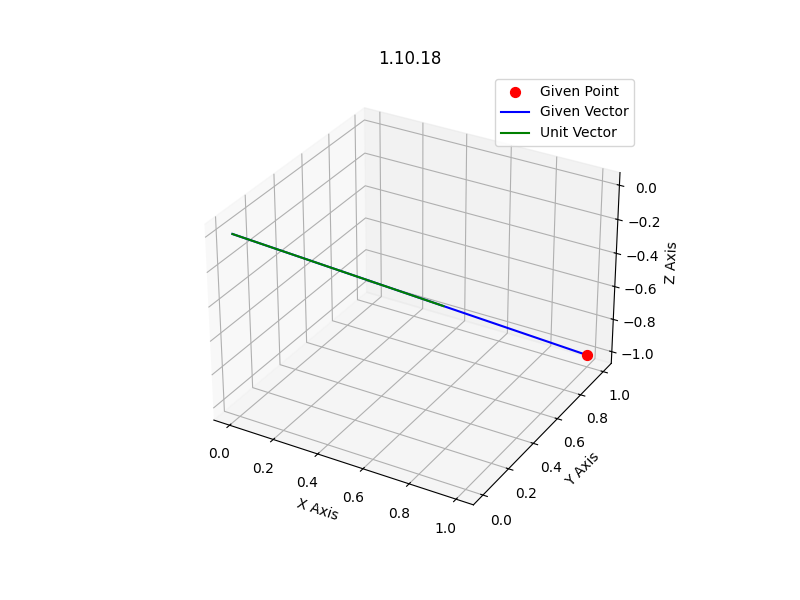
\includegraphics{figs/plot.png}
    \caption*{}
    \label{fig:plot}
\end{figure}
\end{document}
